\documentclass[print]{htwg-report}

% !TEX root = ../report.tex
% Use german umlaute
\usepackage{german,ngerman}
\usepackage[T1]{fontenc}
\usepackage[utf8]{inputenc}
\usepackage[ngerman]{babel}
\usepackage[autostyle=true,german=quotes]{csquotes}

%\usepackage[table]{xcolor}\usepackage{float}
%\usepackage{xcolor,colortbl}

\addbibresource{./bib/report.bib}

\begin{document}

%% Use Roman numerals for the page numbers of the title pages and table of
%% contents.
\frontmatter

%% 'reporttype' add background elements to the cover / front page
%% possible values are:
%% bachelor	--> B S C
%% master	--> M S C
%% other		--> none
\reporttype{bachelor}

\reporttypetext{Bachelor Thesis}

\title[Is it Possible to Write a Sexy Thesis with LaTeX?]{Is it Possible to Write a Sexy Thesis with LaTeX?}

\author{Max Mustermann}
\studentnumber{123456}
\studentemail{Max.Mustermann@htwg.de}
\newcommand{\verfasser}{Max Mustermann}
\newcommand{\thema}{Is it Possible to Write a Sexy Thesis with LaTeX?}
\newcommand{\dob}{01.01.1990}
\newcommand{\birthplace}{Konstanz}
\newcommand{\hoschschule}{Hochschule für Technik, Wirtschaft und Gestaltung}
\newcommand{\institut}{HTWG Konstanz, Institut für Optische Systeme}
\newcommand{\prueferA}{Betreuer A}
\newcommand{\prueferB}{Betreuer B}
\newcommand{\ausgabedatum}{01.04.2019}
\newcommand{\abgabedatum}{01.10.2019}
\newcommand{\type}{Bachelor}
\newcommand{\typeshortcut}{B}
\newcommand{\studiengang}{Angewandte Informatik}
\newcommand{\strasse}{Alfred-Wachtel Straße 11}
\newcommand{\wohnort}{78462 Konstanz}
\newcommand{\schlagworte}{Deep learning, Machine Vision}

\doclocation{Konstanz}
\docdate{01. April 2018}

\makecover[]
%          
%% Include an optional title page.
% !TEX root = report.tex
\begin{titlepage}
\newgeometry{hscale=0.81,vscale=0.8}

\AddToShipoutPicture*{\BackgroundImgTitelPage}

\vspace*{\bigskipamount}


%% Print the title in htwg-teal.
{\makeatletter
\fboxsep=0pt
\colorbox{htwg-white}{\begin{minipage}[t]{145mm}
    \begin{center}
        %% Print Report Type Text
        \color{black}\Huge{\@report@typetext}
        \\
        %% Print Report Title
        \color{black}\Huge\textbf{\@title}
    \end{center}
\end{minipage}}
\makeatother}

\bigskip
\bigskip

{
\setlength{\parskip}{0.5cm}
\begin{center}
	\textbf{zur Erlangung des akademischen Grades}
	
	\textbf{\Large \type\ of Science (\typeshortcut. Sc.)}
	
	\textbf{an der}
	
	\textsf{\huge Hochschule Konstanz}\\
	{\small Technik, Wirtschaft und Gestaltung}
	
    \textsf{\Large Fakultät Informatik} \\
	Studiengang \studiengang
	
\end{center}
}

\bigskip
\bigskip
\bigskip

\begin{center}
	\begingroup
	\renewcommand*{\arraystretch}{1}
	\rowcolors{2}{white}{white}
	{\makeatletter
		\begin{tabular}{lll}
			\type kandidat: & \verfasser \\
							& \strasse \\
							& \wohnort \\ \\ \\ \\
	
			1. Prüfer: & \prueferA \\
			2. Prüfer: & \prueferB \\ \\ \\ \\
			
			Ausgabedatum: & \ausgabedatum \\
			Abgabedatum: & \abgabedatum
		\end{tabular}
		\makeatother}
	\endgroup
\end{center}


%% reset page margins
\newgeometry{hscale=0.7,vscale=0.8}
\end{titlepage}




% !TEX root = report.tex
\chapter*{Abstract}
Ziel des Projekts war das r"aumliche Detektieren eines Modellhubschraubers. Die Detektion soll unter Laborbedingungen stattfinden. Das hei"st, der Helikopter befindet sich vor einer wei"sen Wand.
Zur Lokalisierung des Helikopters im Raum soll zun"achst eine 3D-Punktewolke der Szene generiert und daraus mit Hilfe des Clustering-Algorithmus k-Means die Position des Helikopters bestimmt werden. Auch die Tiefe (Entfernung zur Kamera) des Helikopters soll ermittelt werden. Die Detektion soll mit Hilfe von zwei oder mehr Kameras des Herstellers Point Grey, die "uber eine FireWire-Schnittstelle mit einem Computer verbunden sind, stattfinden.
% !TEX root = report.tex
\chapter*{Extended Abstract}

\begin{center}
	\begingroup
	\renewcommand*{\arraystretch}{1}
	\rowcolors{2}{white}{white}
	{\makeatletter	
		\begin{tabular}{p{3.2cm}p{9.6cm}}
			Thema: & \thema \\
			& \\
			Teammitglieder: & \verfasserA, \verfasserB, 
			\verfasserC, \verfasserD\\
			& \\
			Betreuer: & \hoschschule \newline \institut \newline \prueferA, \prueferB \\
			& \\
		\end{tabular}
		
		\makeatother}
	\endgroup
\end{center}

\bigskip

\noindent
Unser Projekt behandelt das r"aumliche Detektieren eines Modellhubschraubers. Die Detektion soll unter Laborbedingungen, das hei"st, der Helikopter befindet sich vor einer wei"sen Wand, stattfinden. Mittels der Detektion soll auf einem Bild angezeigt werden, wo sich der Mittelpunkt des Helikopters befindet. Auch die Tiefe (Entfernung zur Kamera) des Helikopters soll ermittelt werden. F"ur diese Detektion sollen zwei oder mehr Kameras verwendet werden. Bei diesen handelt es sich um HIERKAMERAEINF"UGEN, die mit dem Computer "uber ein FireWire-Kabel verbunden sind.\newline

\begin{figure}[H]
	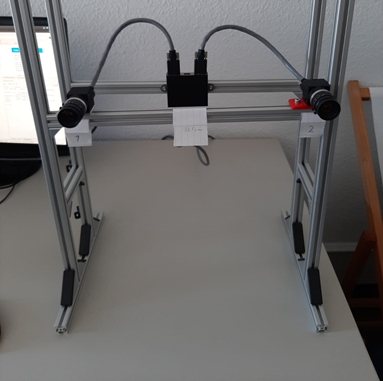
\includegraphics[scale=1.0]{bilder/camerasystem}
	\caption[Kamera-System]{Kamera-System}
\end{figure}

\noindent Das Projekt wurde erfolgreich umgesetzt.
Mittels zwei Kameras, die auf einer geraden Linie angebracht sind, kann der Mittelpunkt des Helikopters und dessen Abstand zur Kamera ermittelt werden.\newline
Unser Programm kalibriert als erstes die Kameras einzeln und anschlie"send zu einander. Das Kalibrieren erfolgt "uber ein Schachbrett-Muster. Sind die Kameras zueinander kalibriert, kann mittels eines Feature-Detektors eine Punktewolke des Helikopters generiert und der Mittelpunkt berechnet werden.

\begin{figure}%
	\centering
	\subfloat[Kamera-Kalibrierung]{{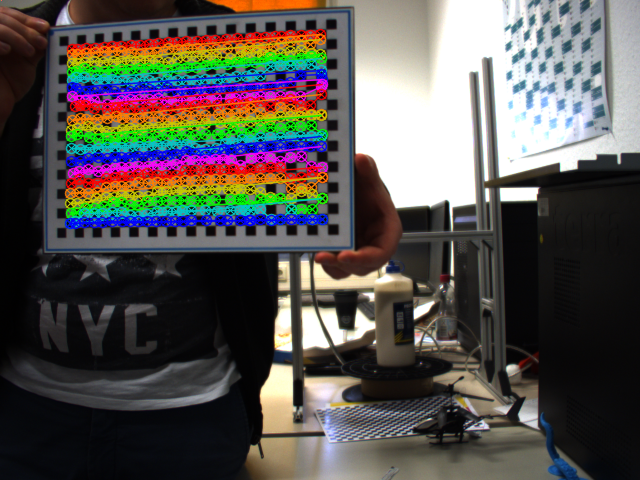
\includegraphics[width=6cm]{bilder/calibration} }}%
	\qquad
	\subfloat[Helikopter-Punktewolke]{{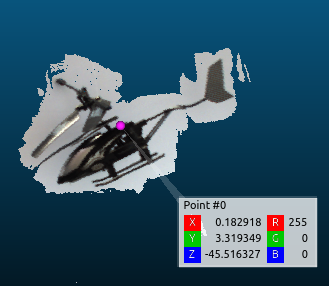
\includegraphics[width=6cm]{bilder/helicloud} }}%
	\caption{Kamera-Kalibrierung und Punktewolke}%
	\label{fig:example}%
\end{figure}
\noindent Eine m"ogliche Erweiterung des Projekts w"are das Kalibrieren von zwei Stereo-Systemen zu einander, um eine noch h"ohere Genauigkeit zu erlangen. Dies wurde versucht umzusetzen, ist allerdings gescheitert.


% !TEX root = report.tex
\chapter*{Ehrenwörtliche Erklärung}
\setheader{Ehrenwörtliche Erklärung}


Hiermit erkläre ich
\textit{\verfasser, geboren am \dob\ in \birthplace}, dass ich\\

\begin{tabular}{lp{12cm}}
\rowcolor{white} (1) & meine Bachelorarbeit mit dem Titel \\[1em]
\rowcolor{white} & \textbf{\thema} \\[1em]
\rowcolor{white} & bei der \hoschschule\ \institut\ unter Anleitung von \prueferA\ selbständig und ohne fremde Hilfe angefertigt und keine anderen als die angeführten Hilfen benutzt habe;\\[1em]
\rowcolor{white} (2) & die Übernahme wörtlicher Zitate, von Tabellen, Zeichnungen, Bildern und
Programmen aus der Literatur oder anderen Quellen (Internet) sowie die Verwendung
der Gedanken anderer Autoren an den entsprechenden Stellen innerhalb der Arbeit
gekennzeichnet habe.\\
\rowcolor{white} (3) & dass die eingereichten Abgabe-Exemplare in Papierform und im PDF-Format vollständig übereinstimmen.\\

\end{tabular}

\vspace*{1cm}

\noindent
Ich bin mir bewusst, dass eine falsche Erklärung rechtliche Folgen haben wird.\\

\vspace*{1cm}

\noindent
Konstanz, \abgabedatum \hfill \begin{tabular}{c} \\ \rowcolor{white} \rule{5cm}{1pt} \\ (Unterschrift)\end{tabular}


\tableofcontents

%% Use Arabic numerals for the page numbers of the chapters.
\mainmatter

% !TEX root = report.tex
\chapter{Introduction}

This document is intended to be both an example of the HTWG Konstanz \LaTeX{} template for reports and theses, as well as a short introduction to its use. It is not intended to be a general introduction to \LaTeX{} itself,\footnote{We recommend \url{http://en.wikibooks.org/wiki/LaTeX} as a reference and a starting point for new users.} and we will assume the reader to be familiar with the basics of creating and compiling documents.


\section{Document Structure}

Since a report, and especially a thesis, might be a substantial document, it is convenient to break it up into smaller pieces. In this template we therefore give every chapter its own file. The chapters (and appendices) are gathered together in \texttt{report.tex}, which is the master file describing the overall structure of the document. \texttt{report.tex} starts with the line
\begin{quote}
    \texttt{\textbackslash documentclass\{htwg-report\}}
\end{quote}
which loads the HTWG Konstanz report template. The template is based on the \LaTeX{} \texttt{book} document class and stored in \texttt{tudelft-report.cls}. The document class accepts several comma-separated options. The default language is English, but this can be changed to Dutch (\emph{e.g.}, for bachelor theses) by specifying the \texttt{dutch} option:
\begin{quote}
    \texttt{\textbackslash documentclass[german]\{htwg-report\}}
\end{quote}
Furthermore, hyperlinks are shown in blue, which is convenient when reader the report on a computer, but can be expensive when printing. They can be turned black with the \texttt{print} option. This will also turn the headers black instead of cyan.

If the document becomes large, it is easy to miss warnings about the layout in the \LaTeX{} output. In order to locate problem areas, add the \texttt{draft} option to the \texttt{\textbackslash documentclass} line. This will display a vertical bar in the margins next to the paragraphs that require attention. Finally, the \texttt{nativefonts} option can be used to override the automatic font selection (see below).

This template has the option to automatically generate a cover page with the \texttt{\textbackslash makecover} command. See the next section for a detailed description.

The contents of the report are included between the \texttt{\textbackslash begin\{document\}} and \texttt{\textbackslash end} commands, and split into three parts by
\begin{enumerate}
\item\texttt{\textbackslash frontmatter}, which uses Roman numerals for the page numbers and is used for the title page and the table of contents;
\item\texttt{\textbackslash mainmatter}, which uses Arabic numerals for the page numbers and is the style for the chapters;
\item\texttt{\textbackslash appendix}, which uses letters for the chapter numbers, starting with `A'.
\end{enumerate}
The title page is defined in a separate file, \emph{e.g.}, \texttt{title.tex}, and included verbatim with \texttt{\textbackslash input\{title\}}.\footnote{Note that it is not necessary to specify the file extension.} Additionally, it is possible to include a preface, containing, for example, the acknowledgements. An example can be found in \texttt{preface.tex}. The table of contents is generated automatically with the \texttt{\textbackslash tableofcontents} command. Chapters are included after \texttt{\textbackslash mainmatter} and appendices after \texttt{\textbackslash appendix}. For example, \texttt{\textbackslash input\{chapter-1\}} includes \texttt{chapter-1.tex}, which contains this introduction.

\section{Bibliography}

The bibliography, finally, is generated automatically with
\begin{lstlisting}
\printbibliography[heading=bibintoc]
\end{lstlisting}
from \texttt{bib/report.bib}. The bibliography style is specified in \texttt{htwg-report.cls}. As an example, we cite the paper by Nobel Prize winner Andre Geim and his pet hamster \cite{Geim2001}. If you need to use a different style, change

\begin{lstlisting}
%% BIB
\RequirePackage[
	backend=biber,
	style=alphabetic,
	sorting=ynt
]{biblatex}
\DefineBibliographyStrings{english}{%
  bibliography = {References},
}
\end{lstlisting}

As compiler, use \texttt{biber} to compile and generate the bibliography.

\section{Cover and Title Page}

This template will automatically generate a cover page if you issue the \texttt{\textbackslash makecover} command. However, before generating the cover, you need to provide the information to put on it. This can be done with the following commands:

\begin{lstlisting}
%% 'reporttype' add background elements to the cover / front page
%% possible values are:
%% bachelor	--> B S C
%% master	--> M S C
%% other		--> none
\reporttype{bachelor}

\reporttypetext{Bachelor Thesis}
\end{lstlisting}

\section{Chapters}

Each chapter has its own file. For example, the \LaTeX{} source of this chapter can be found in \texttt{chapter-1.tex}. A chapter starts with the command
\begin{quote}
    \texttt{\textbackslash chapter\{Chapter title\}}
\end{quote}
This starts a new page, prints the chapter number and title and adds a link in the table of contents. If the title is very long, it may be desirable to use a shorter version in the page headers and the table of contents. This can be achieved by specifying the short title in brackets:
\begin{quote}
    \texttt{\textbackslash chapter[Short title]\{Very long title with many words which could not possibly fit on one line\}}
\end{quote}
Unnumbered chapters, such as the preface, can be created with \texttt{\textbackslash chapter*\{Chapter title\}}. Such a chapter will not show up in the table of contents or in the page header. To create a table of contents entry anyway, add
\begin{quote}
    \texttt{\textbackslash addcontentsline\{toc\}\{chapter\}\{Chapter title\}}
\end{quote}
after the \texttt{\textbackslash chapter} command. To print the chapter title in the page header, add
\begin{quote}
    \texttt{\textbackslash setheader\{Chapter title\}}
\end{quote}

Chapters are subdivided into sections, subsections, subsubsections, and, optionally, paragraphs and subparagraphs. All can have a title, but only sections and subsections are numbered. As with chapters, the numbering can be turned off by using \texttt{\textbackslash section*\{\ldots\}} instead of \texttt{\textbackslash section\{\ldots\}}, and similarly for the subsection.
\section{\textbackslash section\{\ldots\}}
\subsection{\textbackslash subsection\{\ldots\}}
\subsubsection{\textbackslash subsubsection\{\ldots\}}
\paragraph{\textbackslash paragraph\{\ldots\}}
Lorem ipsum dolor sit amet, consectetur adipisicing elit, sed do eiusmod tempor incididunt ut labore et dolore magna aliqua. Ut enim ad minim veniam, quis nostrud exercitation ullamco laboris nisi ut aliquip ex ea commodo consequat. Duis aute irure dolor in reprehenderit in voluptate velit esse cillum dolore eu fugiat nulla pariatur. Excepteur sint occaecat cupidatat non proident, sunt in culpa qui officia deserunt mollit anim id est laborum.

\section{Fonts and Colors}

If you want to use the HTWG house style font \texttt{Swiss 721} it is necessary to put the font as \texttt{.ttf} file under \texttt{fonts}. As fallback font \texttt{Arial} is used. For more informations to the HTWG house style font see \url{https://www.htwg-konstanz.de/hochschule/einrichtungen/stabsstelle-kommunikation/corporate-design-logo/}.




%% Use letters for the chapter numbers of the appendices.
\appendix

%\input{appendix-a}

\printbibliography[heading=bibintoc]

\end{document}

